The implementation, integration and test plan will follow a \textbf{bottom-up approach},
starting from the components with no dependencies and then integrating them together.

\section{Plan Definition}
Since the application is mostly server-side, we will only describe the implementation of the server components.
The client-side, which is actually a presentation layer, will be implemented and tested in parallel with the server-side.

Since our application is developed on two different servers, we will describe separately 
the implementation plan for the two servers: the \textit{CKB Server} and the \textit{Evaluation Server}.
\subsubsection{CKB Server}

In the first step, the \textit{Model} (under the specified assumption of \textit{MVC pattern}) and the \textit{Data Manager}, will be implemented and unit
tested with a \textit{Driver} which will substitute components which are not already implemented.

\begin{figure}[H]
    \label{fig:step1-CKBServer}
    \centering
    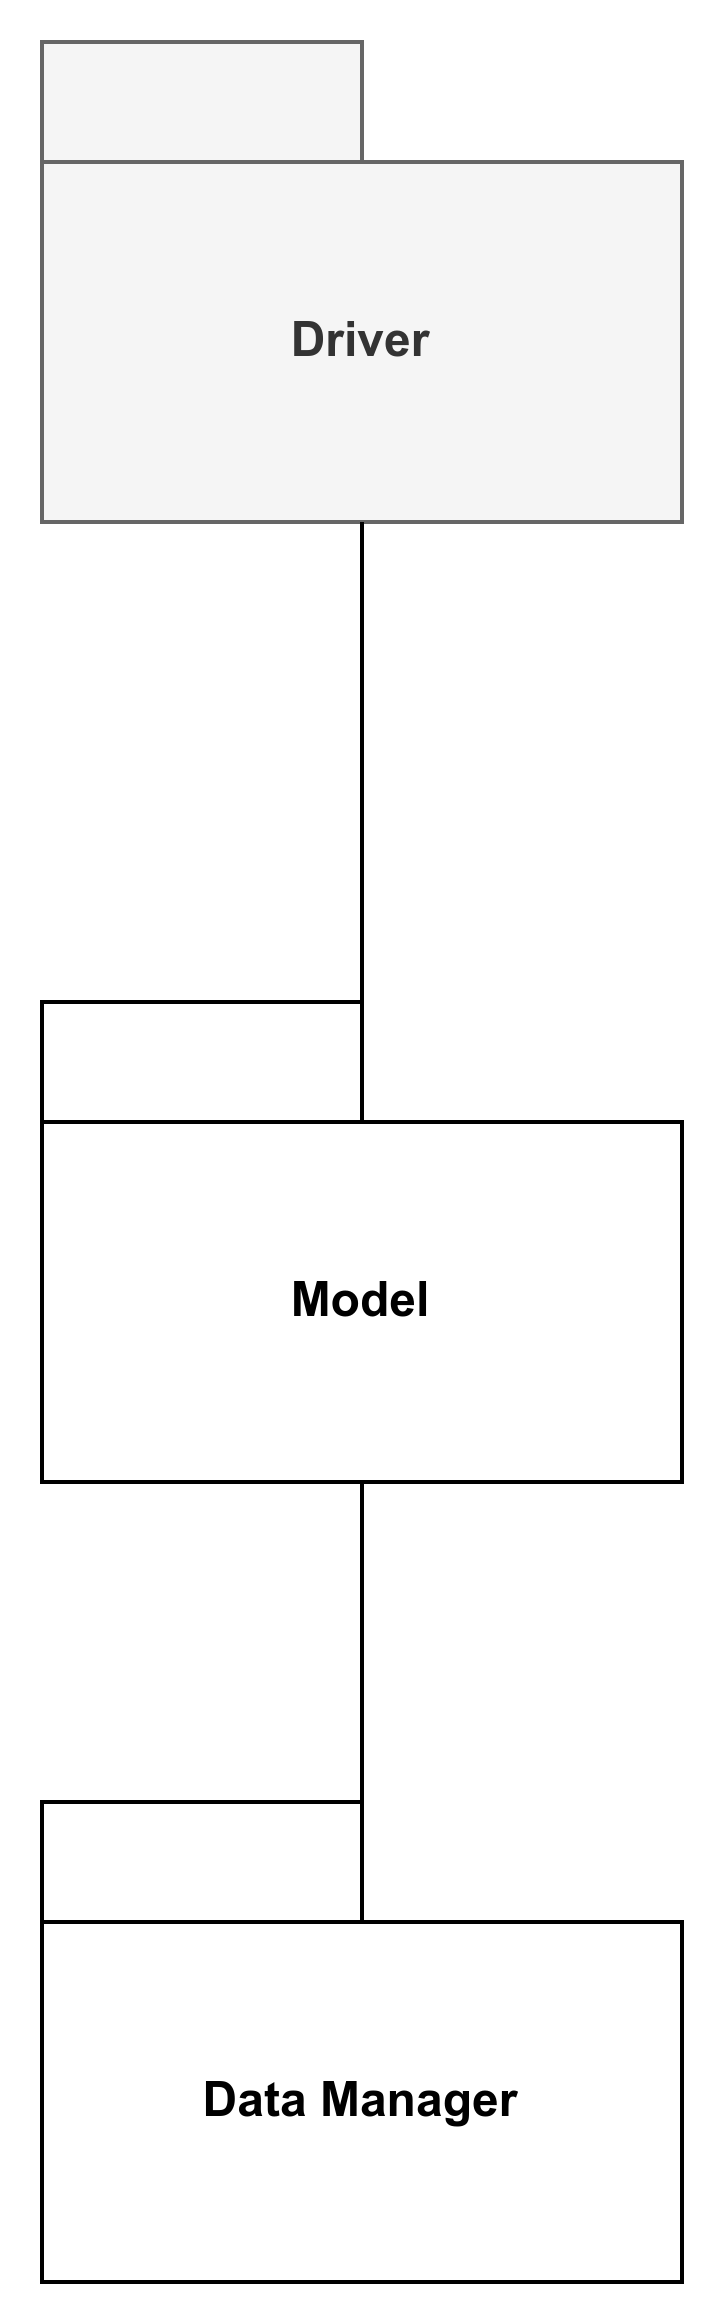
\includegraphics[height=0.5\textheight]{ImplementationStrategy/1_01-CKBServer.png}
    \caption{Step 1}
\end{figure}
\pagebreak

In the second step, the Notification Manager will be implemented and tested with a \textit{Driver} which will substitute: 
the \textit{Competition Manager},the \textit{Battle Manager} and the \textit{Authentication Service}.
It will also use a \textit{Stub} to simulate the \textit{Mail Server}.
\begin{figure}[H]
    \label{fig:step2-CKBServer}
    \centering
    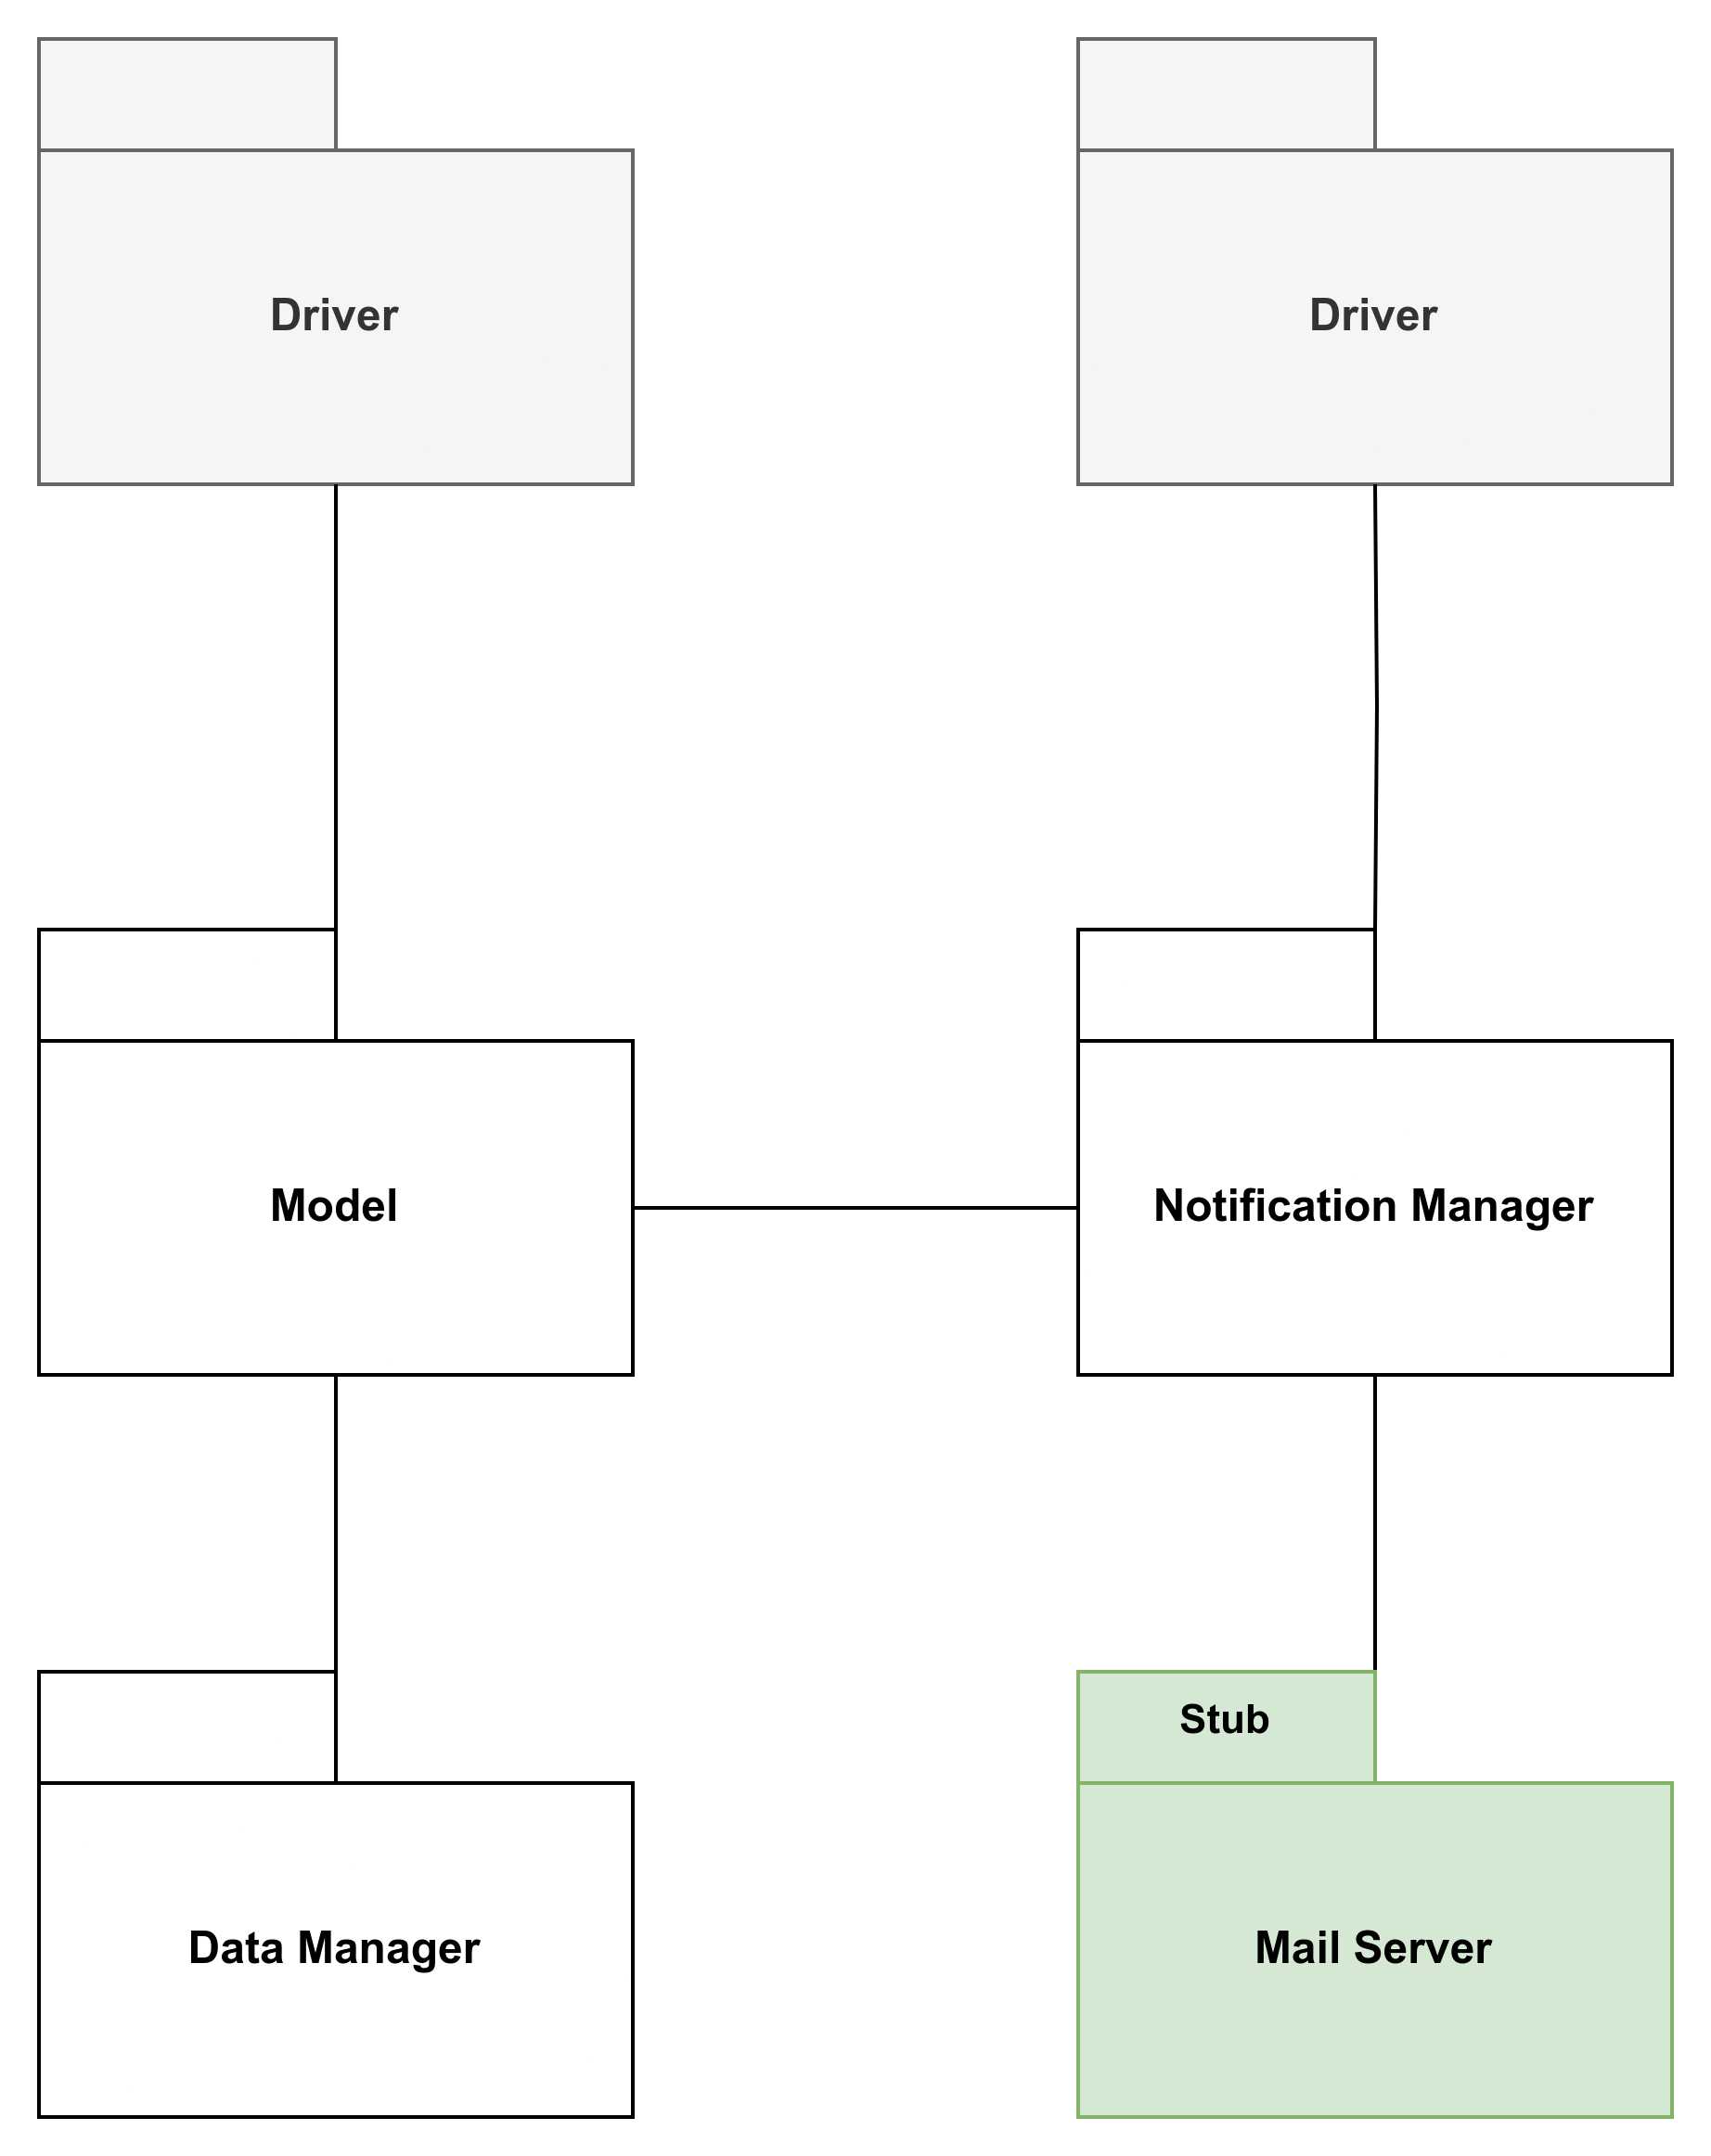
\includegraphics[height=0.5\textheight]{ImplementationStrategy/1_02-CKBServer.png}
    \caption{Step 2 - CKB Server}
\end{figure}
\pagebreak

In the third step, the Authentication Service will be implemented and tested, a \textit{Driver} will substitute the \textit{Dashboard Manager}.
\begin{figure}[H]
    \label{fig:step3-CKBServer}
    \centering
    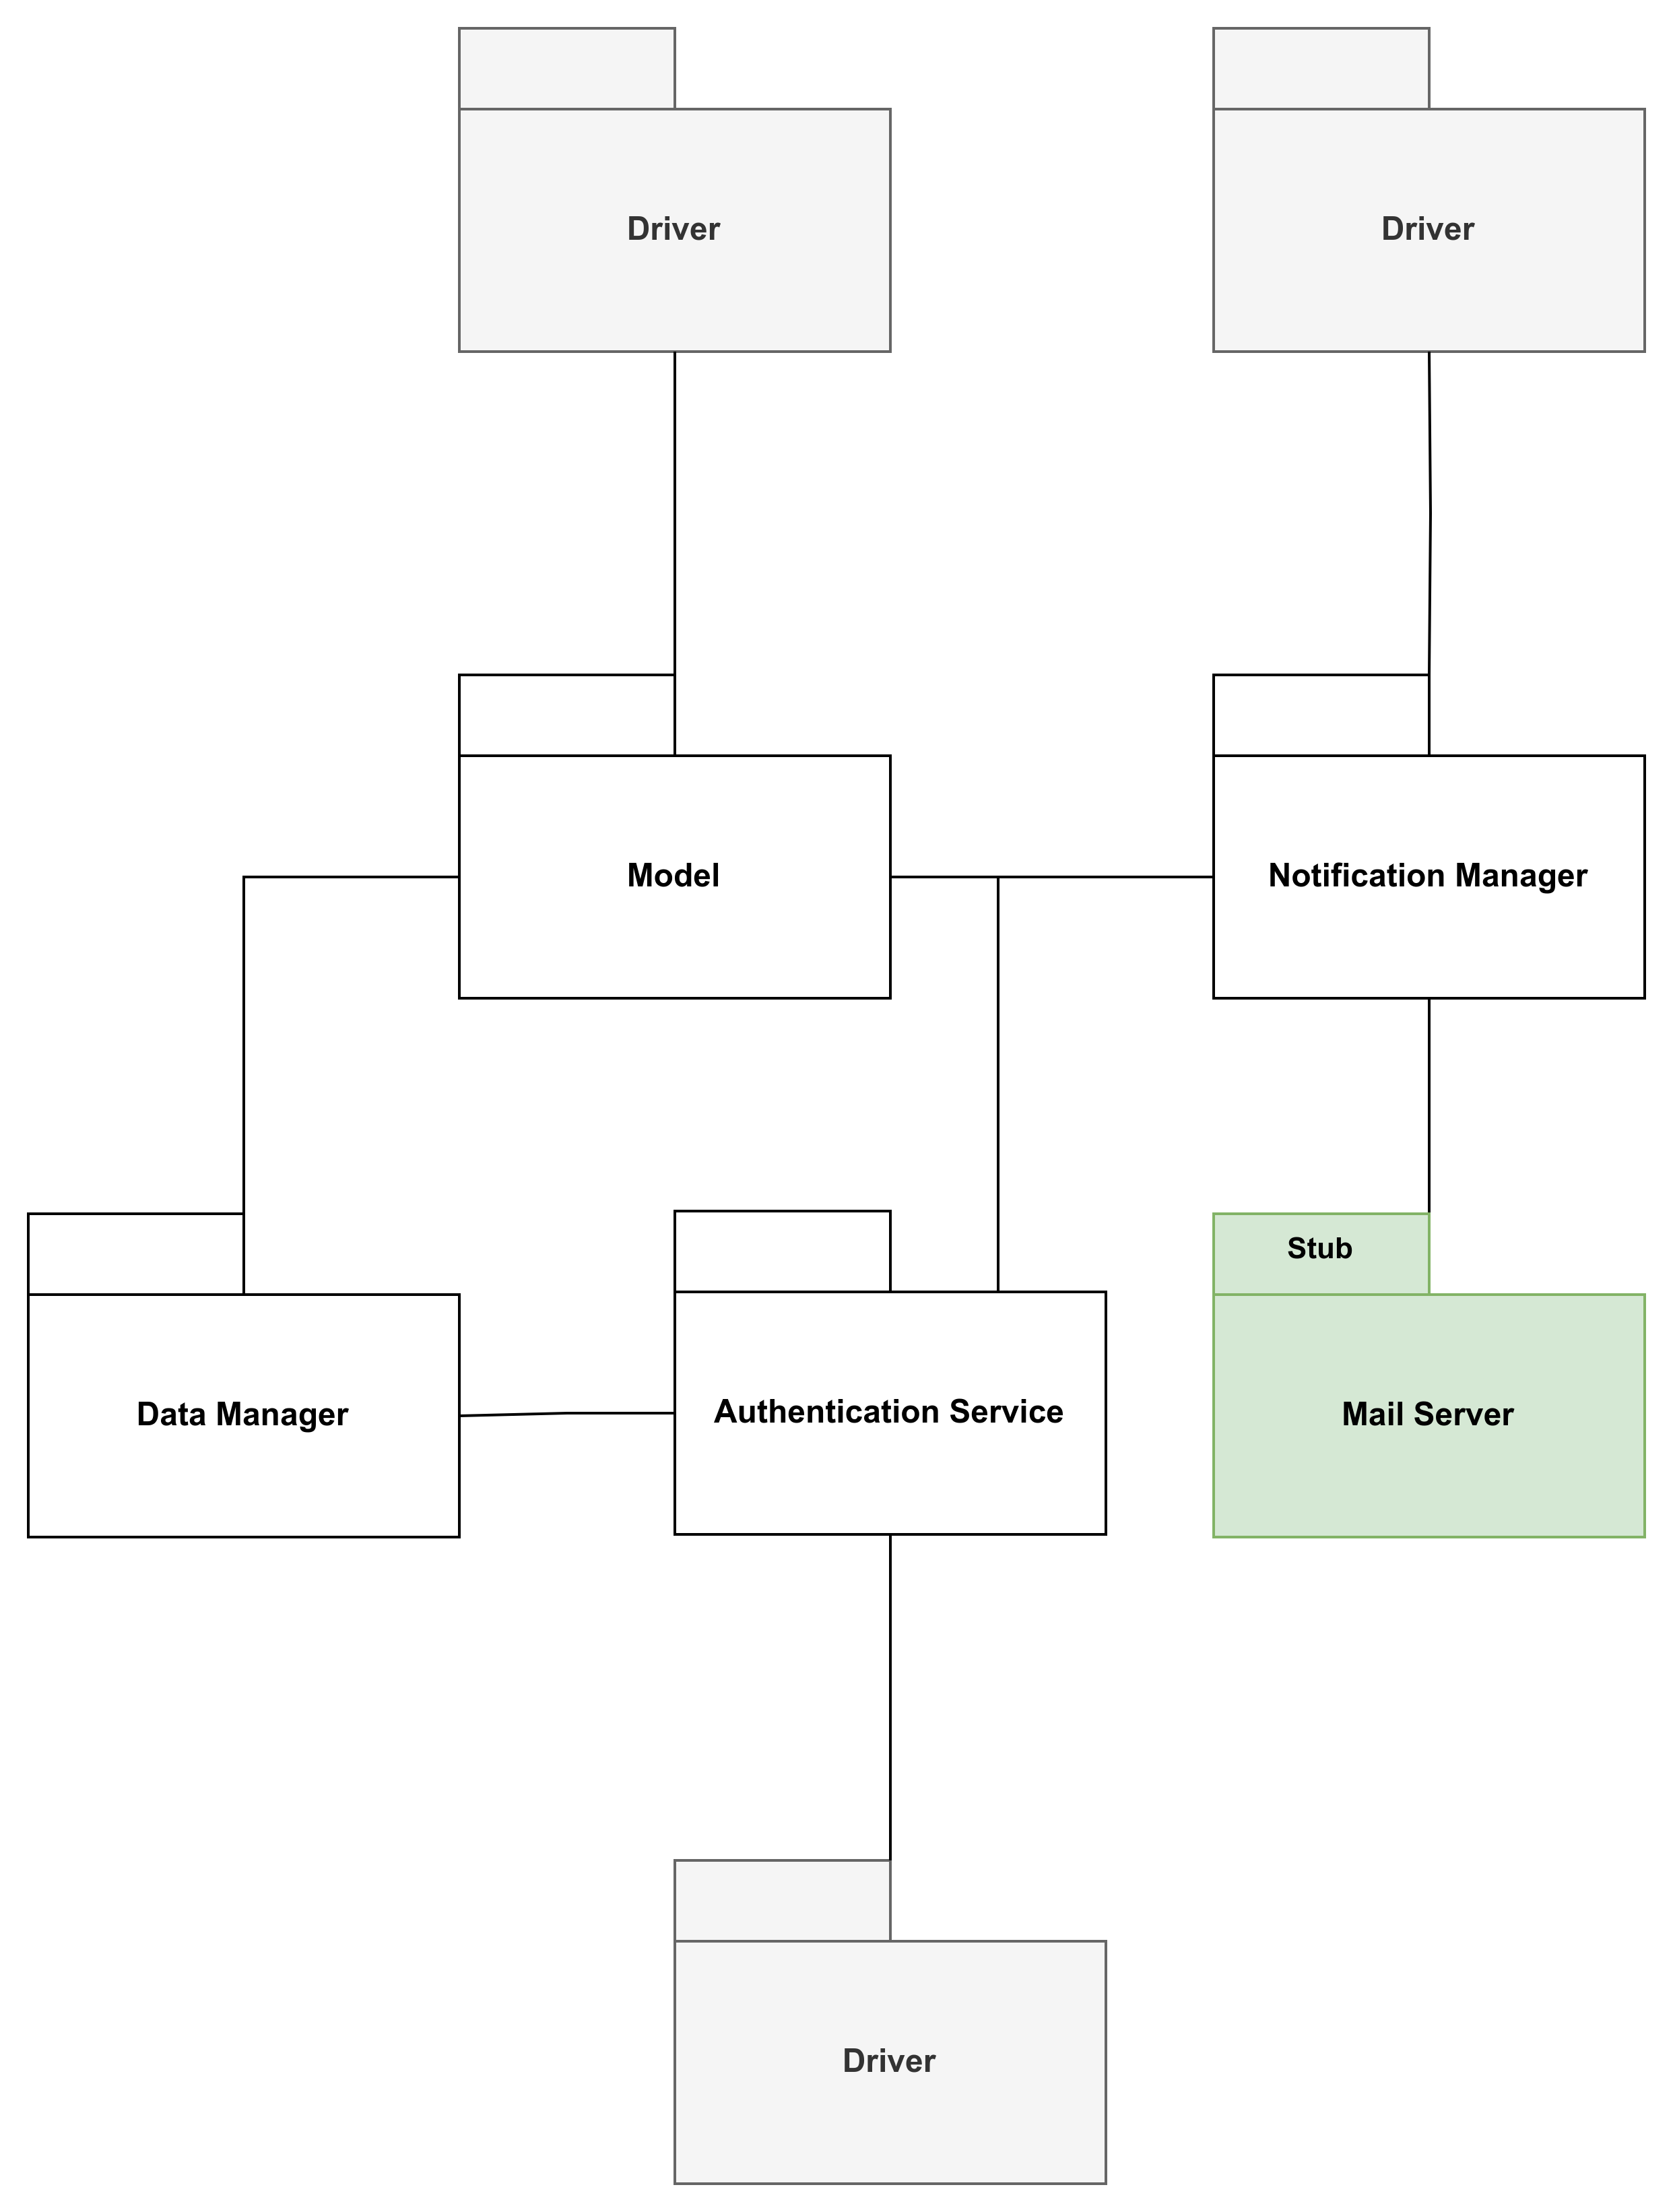
\includegraphics[height=0.5\textheight]{ImplementationStrategy/1_03-CKBServer.png}
    \caption{Step 3 - CKB Server}
\end{figure}
\pagebreak
In the fourth step, the \textit{Competition Manager}, the \textit{Battle Manager}, the \textit{Team Manager}
and the \textit{Badge Manager} and the will be implemented and tested in parallel, a \textit{Driver} will substitute the \textit{Dashboard Manager}.
\begin{figure}[H]
    \label{fig:step4-CKBServer}
    \centering
    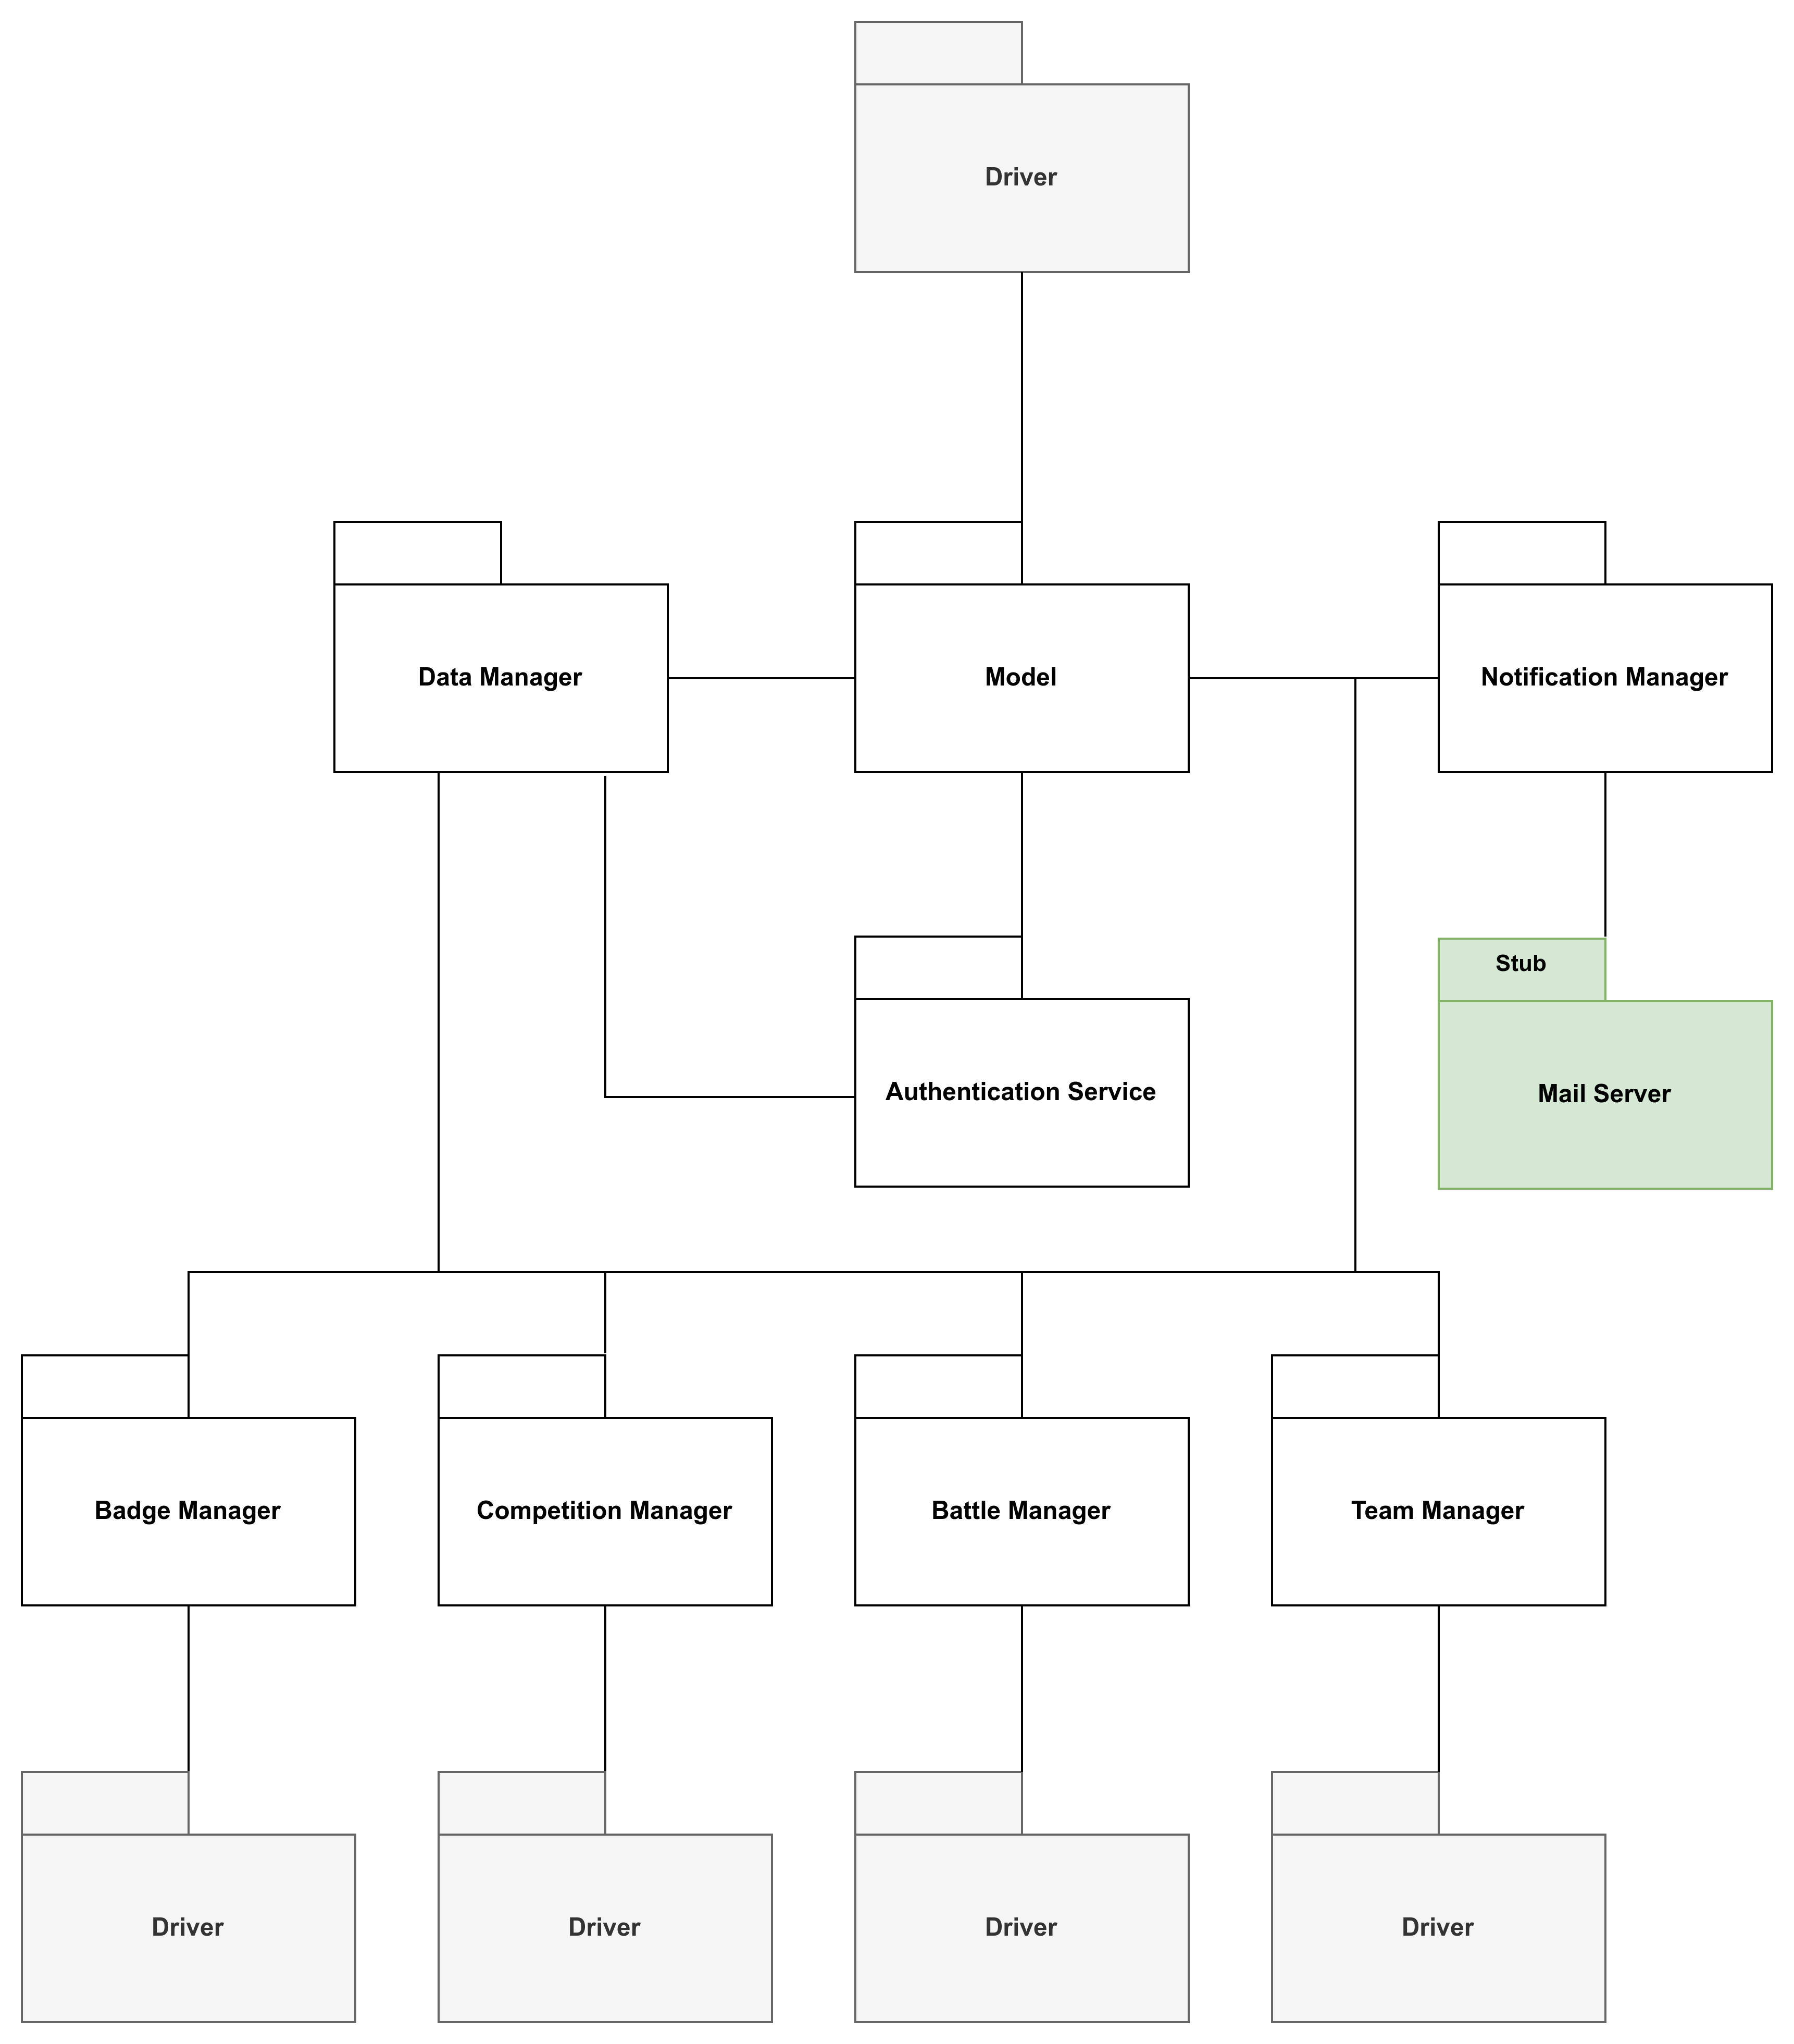
\includegraphics[height=0.8\textheight]{ImplementationStrategy/1_04-CKBServer.png}
    \caption{Step 4 - CKB Server}
\end{figure}
\pagebreak

\begin{figure}[H]
    \label{fig:step5-CKBServer}
    \centering
    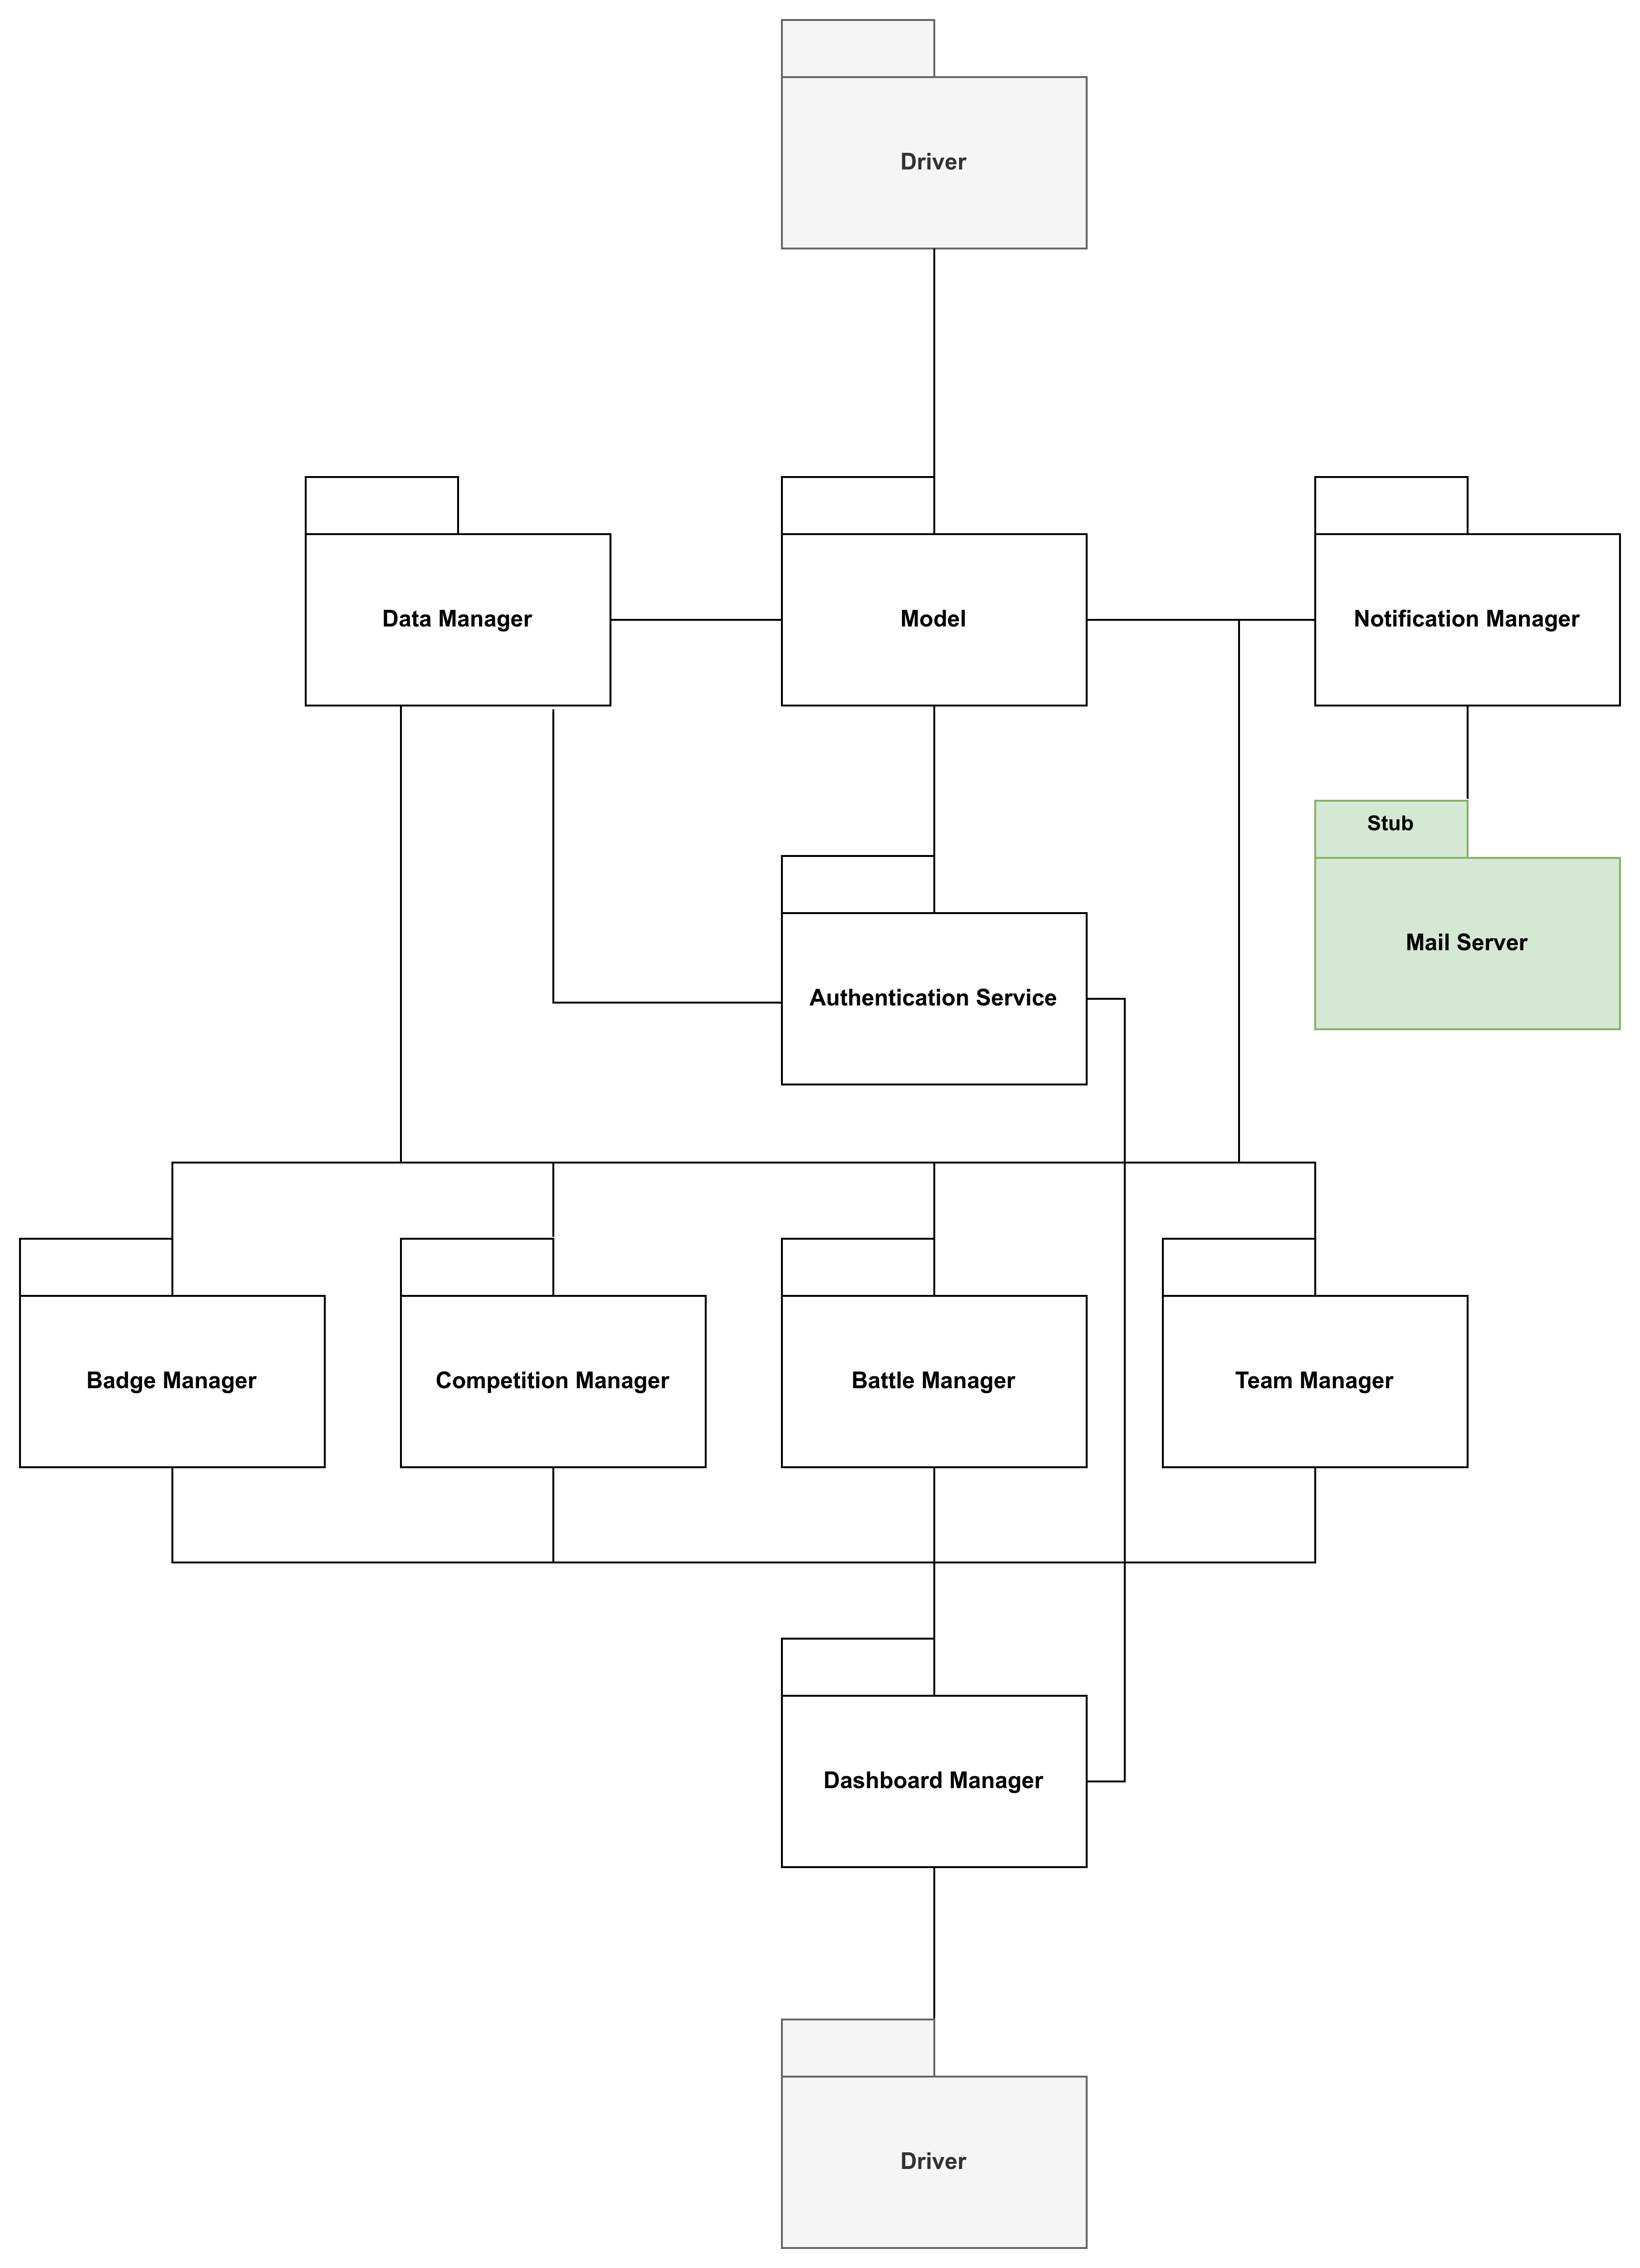
\includegraphics[height=0.8\textheight]{ImplementationStrategy/1_05-CKBServer.png}
    \caption{Step 5 - CKB Server}
\end{figure}
\pagebreak

\subsubsection{Evaluation Server}

\begin{figure}[H]
    \label{fig:step1-EvaluationServer}
    \centering
    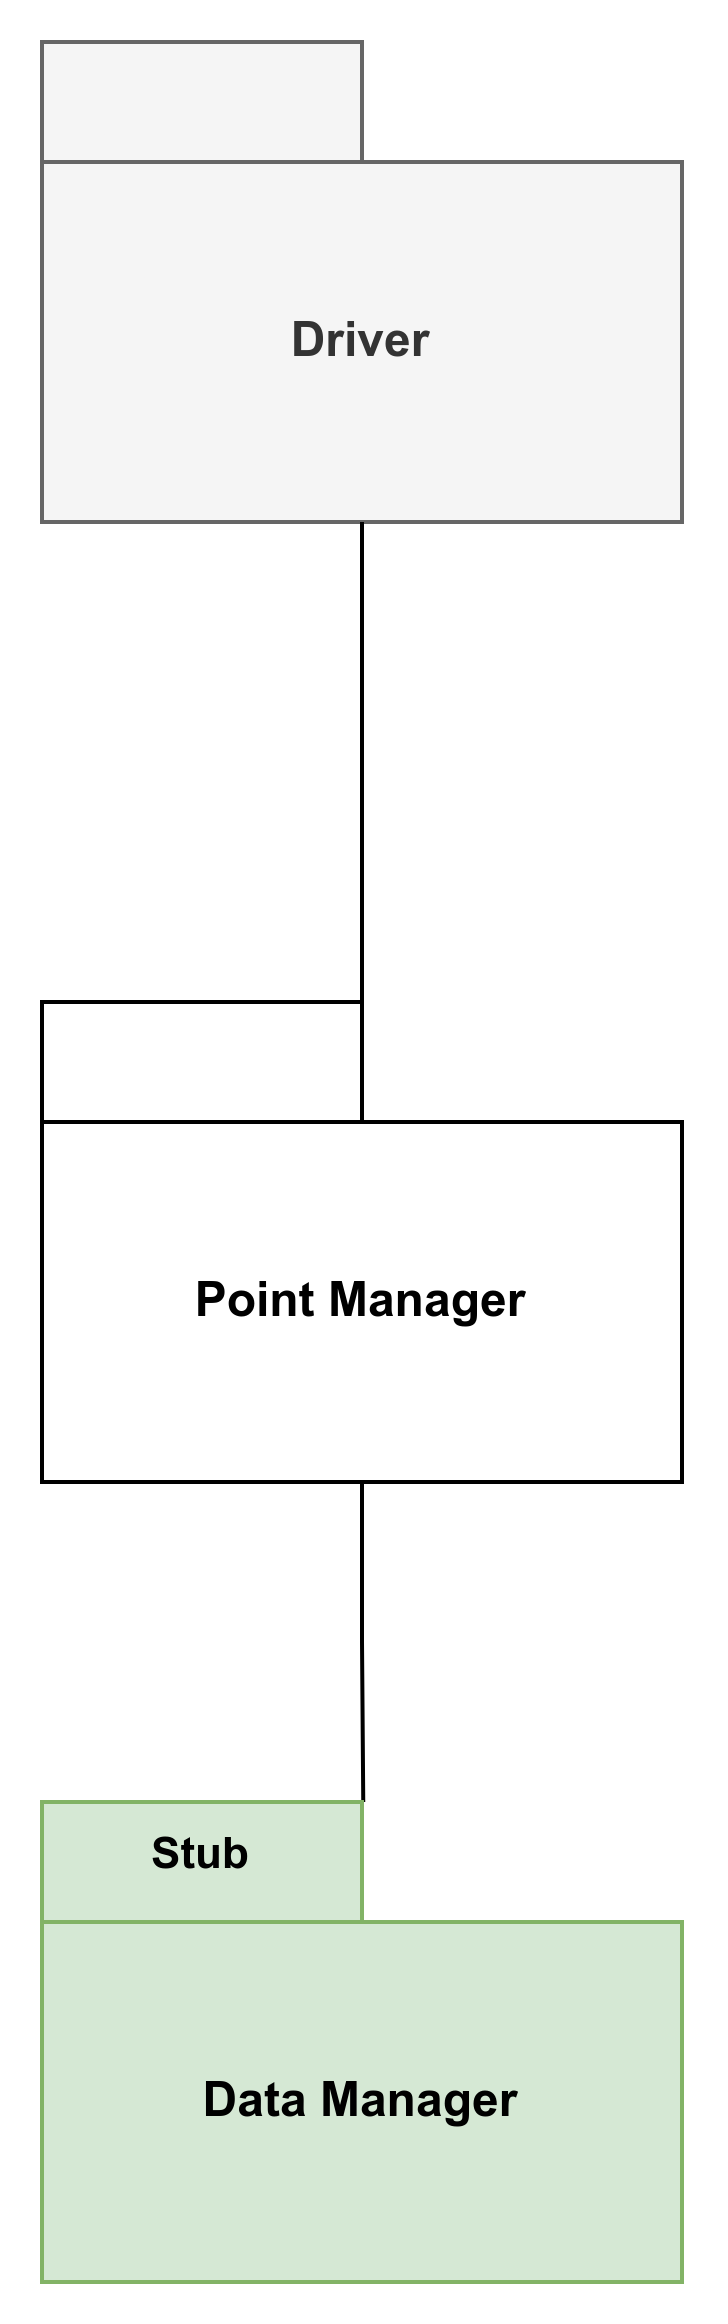
\includegraphics[height=0.5\textheight]{ImplementationStrategy/2_01-EvaluationServer.png}
    \caption{Step 1 - Evaluation Server}
\end{figure}

\begin{figure}[H]
    \label{fig:step2-EvaluationServer}
    \centering
    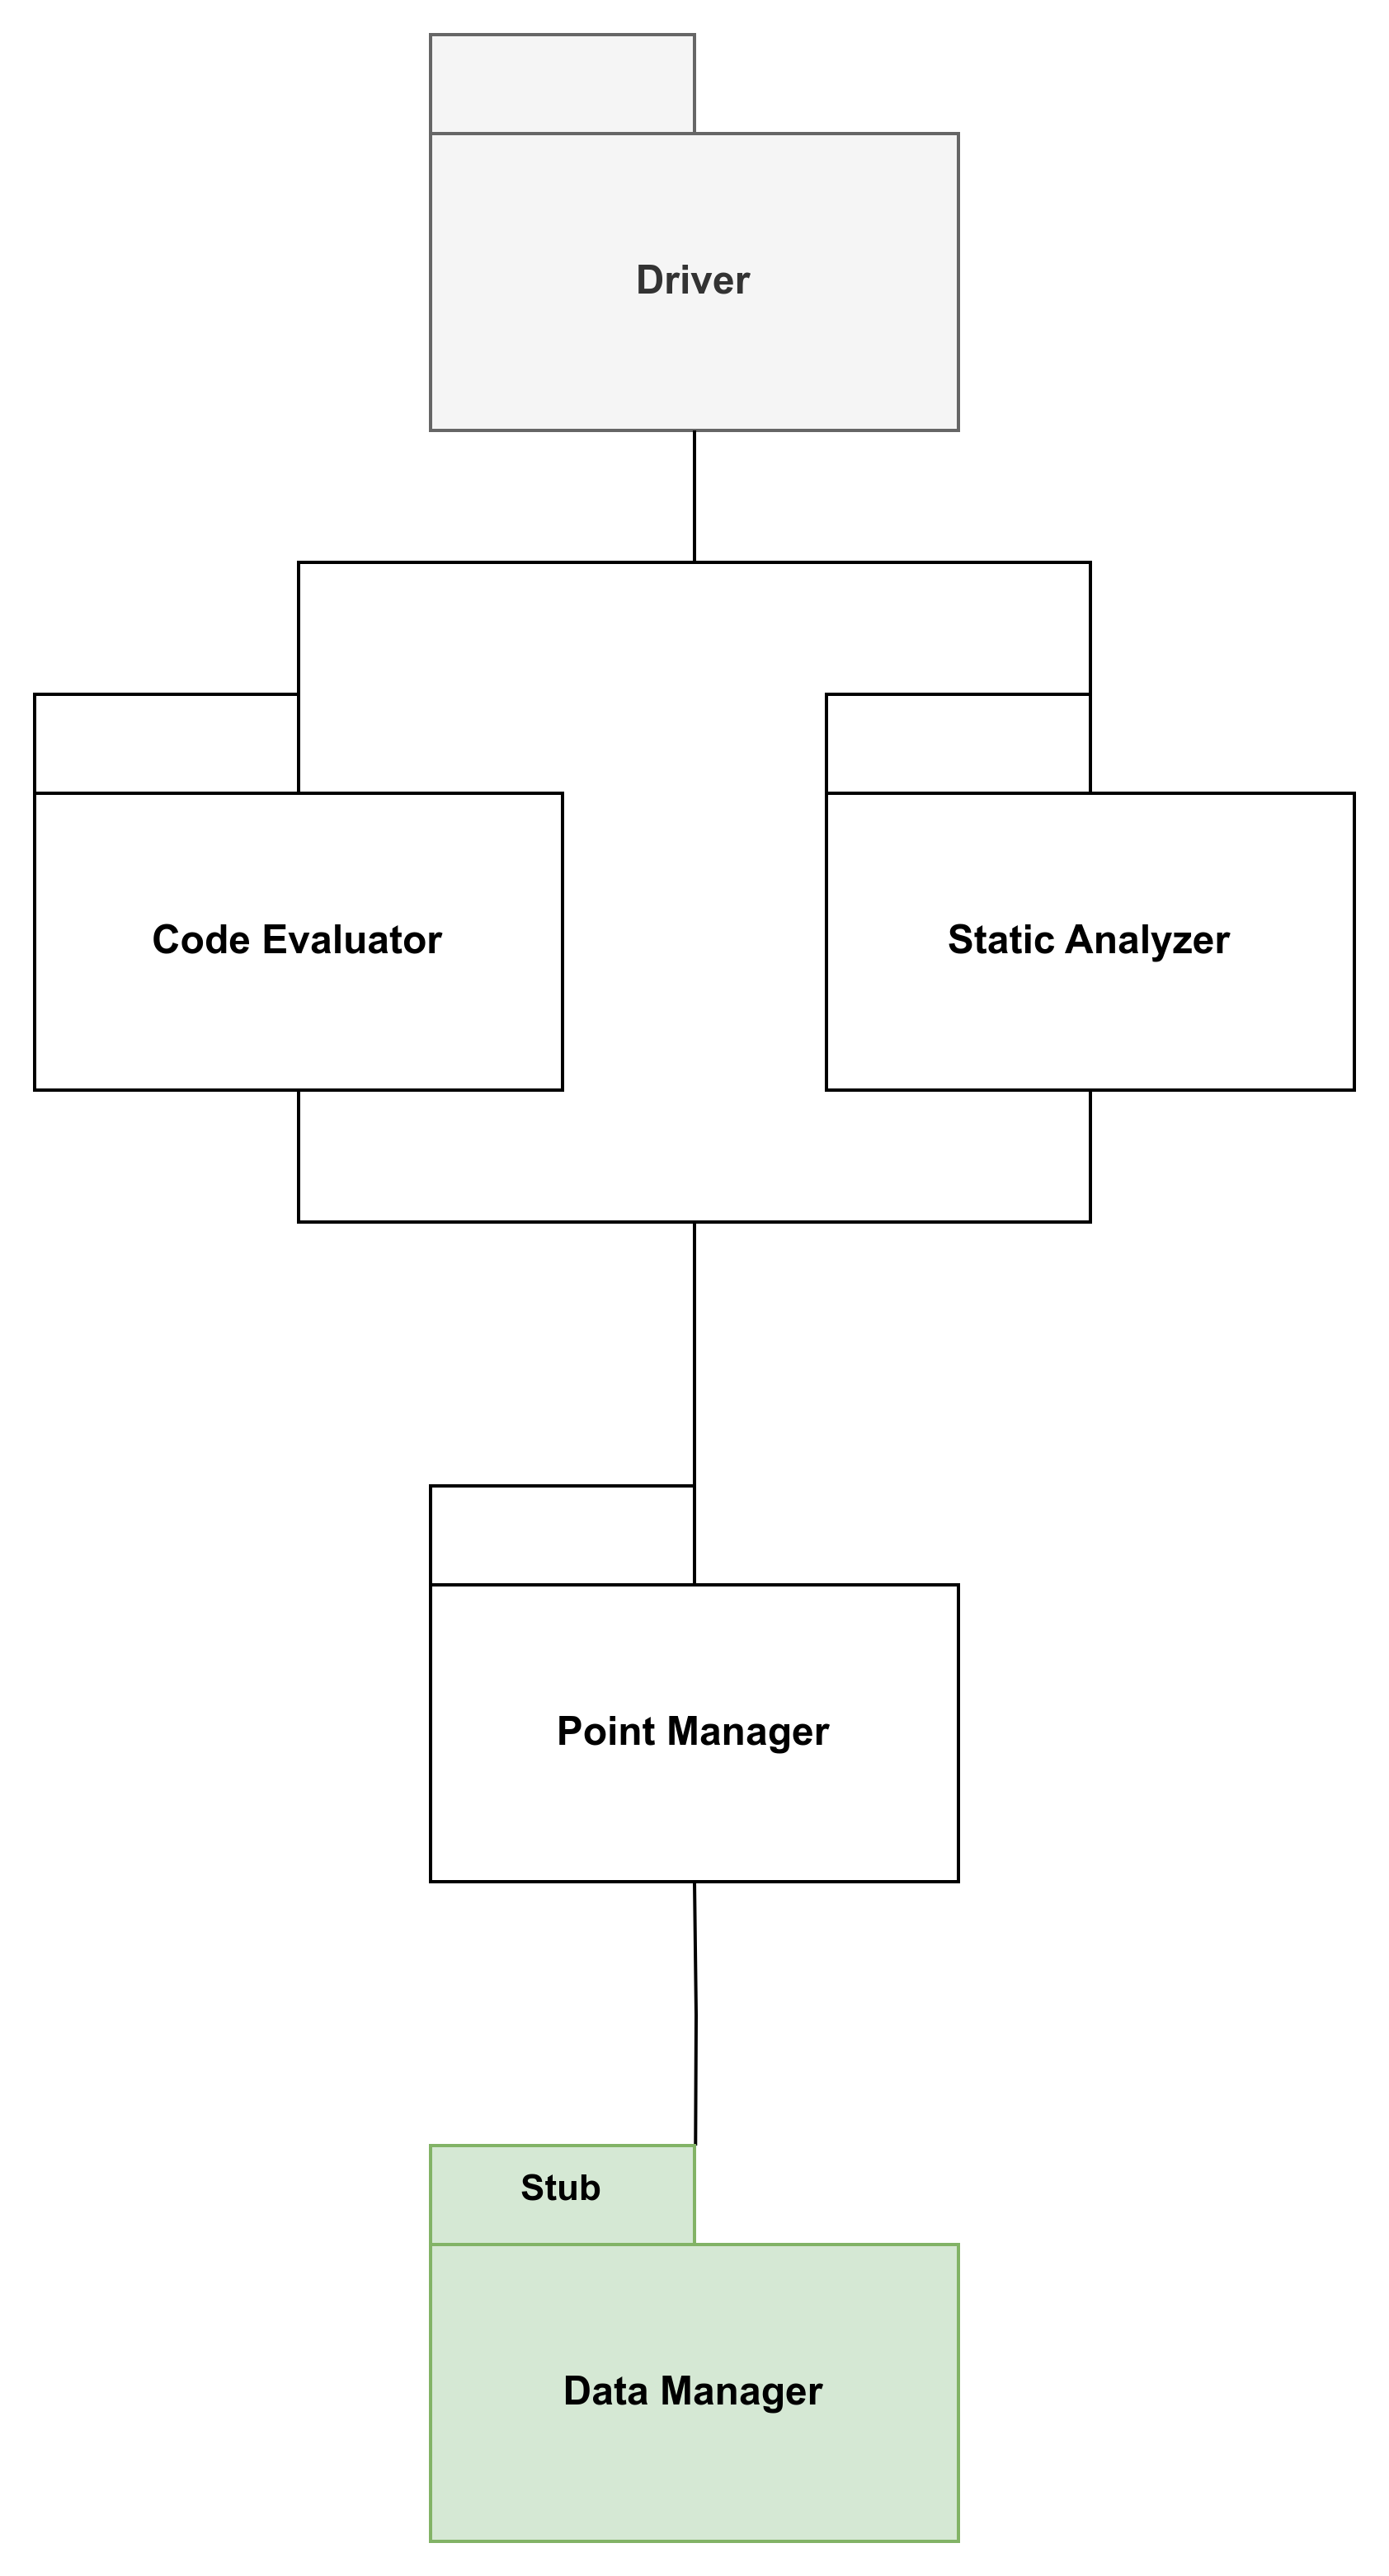
\includegraphics[height=0.5\textheight]{ImplementationStrategy/2_02-EvaluationServer.png}
    \caption{Step 2 - Evaluation Server}
\end{figure}

\begin{figure}[H]
    \label{fig:step3-EvaluationServer}
    \centering
    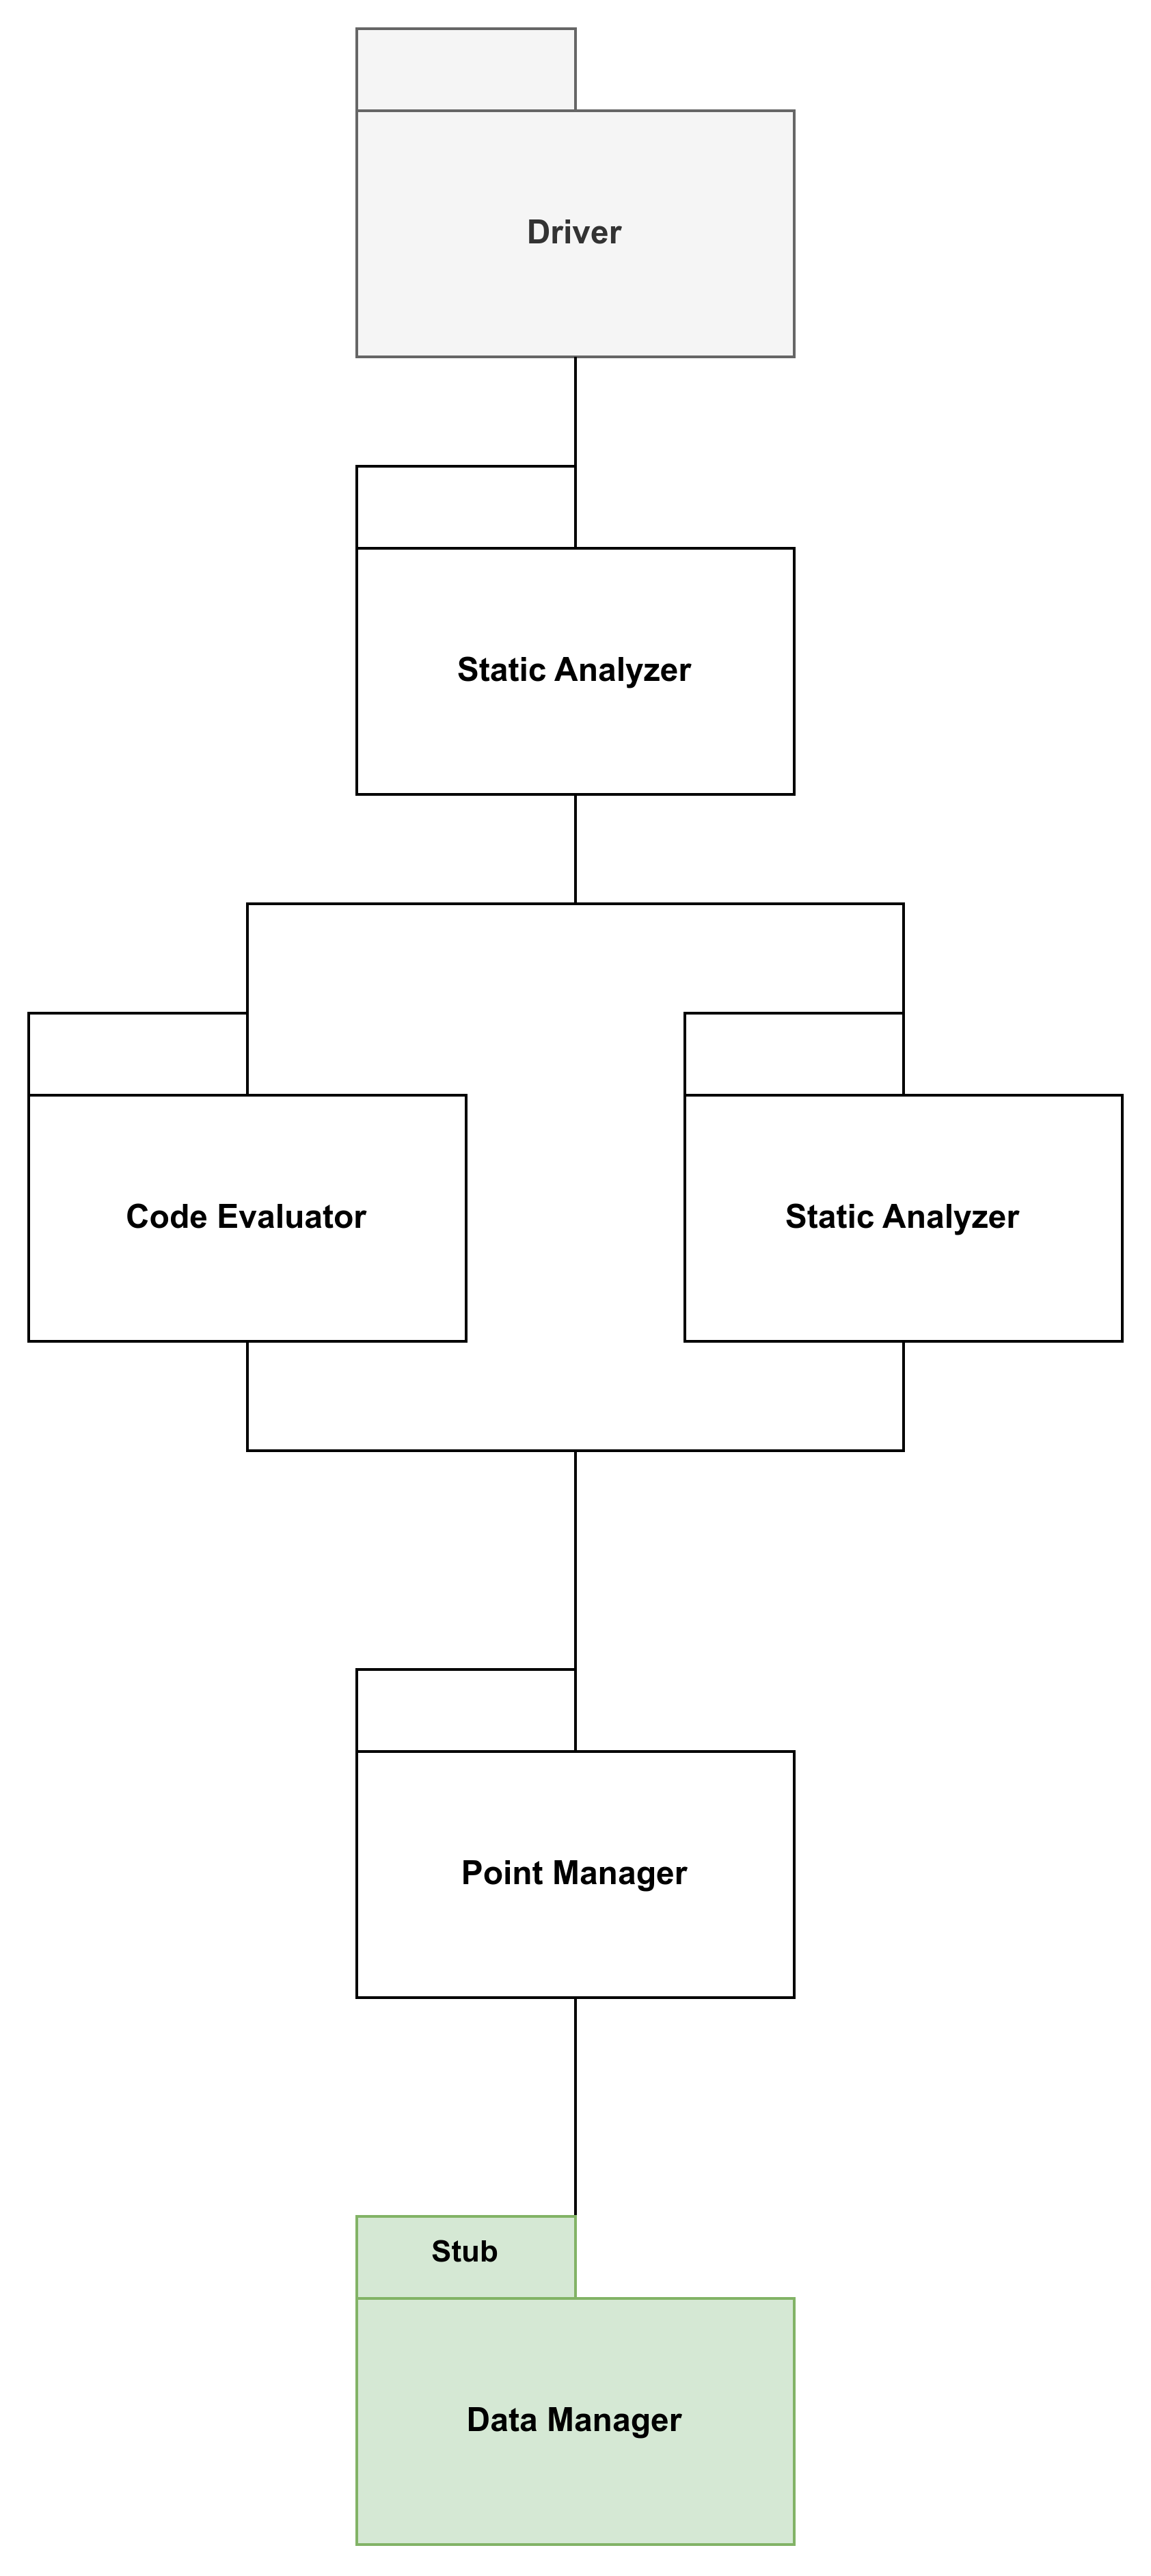
\includegraphics[height=0.5\textheight]{ImplementationStrategy/2_03-EvaluationServer.png}
    \caption{Step 3 - Evaluation Server}
\end{figure}
